\documentclass{article}

\usepackage[utf8]{inputenc}
\usepackage[english]{babel}
\usepackage{mathrsfs,amsmath}
\usepackage{nonfloat}
\usepackage{float}
\usepackage{graphicx}
\usepackage{subfig}


% Puts captions of tables on top
\floatstyle{plaintop}
\restylefloat{table}

% Puts captions in bold
\captionsetup{labelfont=bf}

\begin{document}

\section{Introduction of Centroid Computing}

Centroid computing is a process of calculating the center of intensities, with prior knowledge of number of lenslets and the position of ideal spots. The position of the ideal spots is the centroid position of a non-aberrated wave-front intensities. When the wave-front is aberrated, the centroid result will differ from the ideal spots (see figure~\ref{fig:fig1}). Calculating the error from the centroids measured to the ideal spots is the main principle of centroid computing. After knowing the error, the next process is calculating the slopes of the wave-front, which later will be used in wave-front reconstruction process.

\begin{figure}[H]
    \centering
    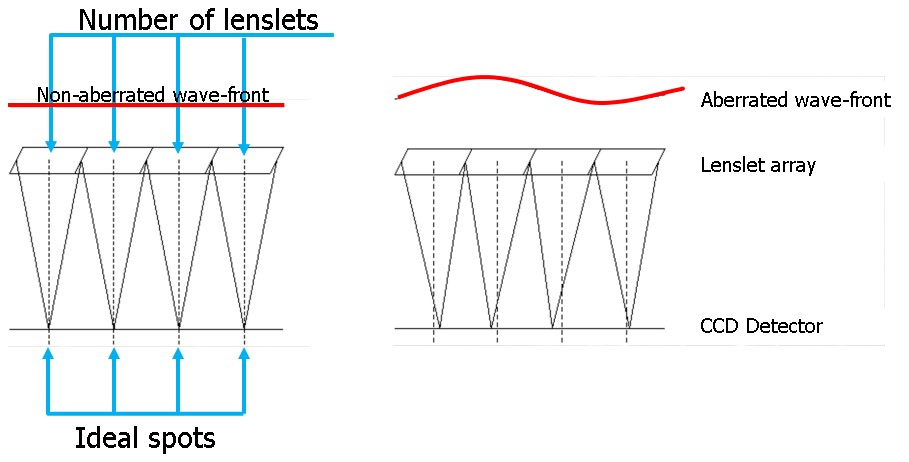
\includegraphics[width=4in]{figures/fig1.jpg}
    \caption{The difference between aberrated and non-aberrated wave-front centroid position}
    \label{fig:fig1}
\end{figure}

A Shack-Hartmann Wavefront sensor samples the incident wavefront by means of a lenslet array which produces an array of spots on a detector. The wavefront is then analyzed by measuring, in real time, the displacement of the centroids of those spots. The Shack-Hartmann Wavefront sensor has been a popular choice for any Adaptive Optics (AO) system. One of the factor that determines the performance of the Shack-Hartmann Wavefront sensor is its accuracy, which depends on whether it has accurate estimation and robust centroid algorithm. Therefore, determining which algorithm has accurate estimation and robust under different conditions of photon flux, read-out noise (RON), and sampling is very crucial.

In Adaptive Optic used in telescope, centroid computing is corrupted by the coarse sampling of the CCD, photon noise, read-out noise (RON) of the CCD, and speckle noise introduced by the atmosphere. All of those factors can determine which method is better, in accurate estimation and robustness, than the others based on the specific condition of those factors. It is crucial because if we do not carefully consider those factors, we will end up getting wrong centroid result.

In case of strong RON and weak signal, for example, the spot is completely lost in the detector noise. This is crucial problem if we use the method that rely on the brightest pixel(s) to determine the center of the spot, like tresholding method for example. Since the spot is completely lost (not detected), the centroid calculation from this method will get wrong result.

The photon noise and the read-out noise are uncorrelated, so there is no cross-correlation between them. Therefore, the formula to calculate the total centroid measuring error $\sigma_{err}^2$ is:

\begin{equation}
\sigma_{err}^2 =\sigma_{ph}^2+\sigma_r^2
\end{equation}
where $\sigma_{ph}^2$ is the photon noise and $\sigma_{r}^2$ is the read-out noise (RON). 

The lower boundary of the centroid error is reached in the case of pure photon noise and a gaussian spot,

\begin{equation}
\sigma_{err} = \frac{\sigma}{\sqrt{N_{ph}}}
\end{equation}
where $\sigma$ is the rms size of the spot and $N_{ph}$ is the number of photons. This boundary is reached by simple centroid, he optimum method for no RON. However, existing RON will make other methods superior, because of the existence of diffraction of the spot.

Some of the methods to compute centroid are explained below.

\section{Centroid Algorithm Methods}

\subsection{Thresholding}

In thresholding method, the significant pixels, or the pixels which are included on the mean calculation, are chosen considering their intensity relative to the maximum intensity (brightest pixel(s)). Therefore, as has been stated before, thresholding methos rely on the brightest pixel(s) to determine the center.

\begin{figure}[H]
    \centering
    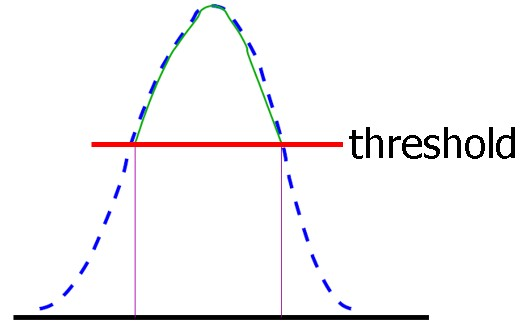
\includegraphics[width=2.5in]{figures/threshold.jpg}
    \caption{The thresholding method principle}
    \label{fig:threshold}
\end{figure}

Firstly, the pixel(s) with maximum intensity ($I_{max}$) is determined, then the threshold ($C$) is set at $T.I_{max}$, where $T$ is the threshold value. But, the threshold should be no less than $3.N_r$ ($N_r$ = Readout Noise). Choosing $3.N_r$ as a lower bound for setting the threshold has advantage for low SNR since it will removes most of the noisy pixels without removing the signal itself~\cite{thomas04}.

After determining the pixel(s) with maximum intensity and the threshold, it is obviously easy to know which pixels should be included in the centroid calculation. After knowing that information, finally, the simple center of gravity calculation can be used to determine the centroid location.

\subsection{Windowing}

This windowing method has almost same principles with thresholding method unless for the determining which pixels should be included in centroid calculation. The thresholding method uses thresholding which is determined from $T.I_{max}$, while the windowing uses a circular window. 

\begin{figure}[H]
    \centering
    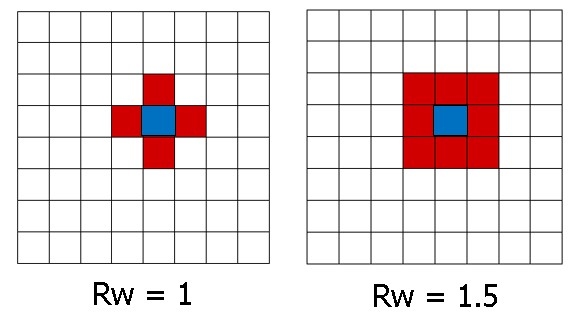
\includegraphics[width=2.5in]{figures/window.jpg}
    \caption{The windowing method principle}
    \label{fig:window}
\end{figure}

The circular window defines which pixels will be included into the centroid calculation. The principle is simply by defining $W(r)=1$ for $r<R_w$ and $W(r)=0$ otherwise, with $R_w$ is the radius of the window. The center of the window is determined by the maximum intensity pixel(s) just the same as threshold method.

And the same with thresholding, simple center of gravity algorithm can be used to determine the centroid after knowing which pixels is inside the window.

\subsection{Correlation}

This method calculates the correlation between the image obtained by the CCD and a reference spot (template) \cite{poyneer03}. The template used is a 2D Gaussian function with certain rms size $\sigma$. Then we can use the simple centroid calculation / center of gravity to calculate the centroid based on those correlation.

\begin{figure}[H]
\begin{minipage}[t]{0.3\textwidth}
\centering
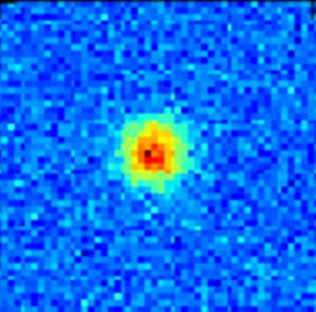
\includegraphics[width=\linewidth]{figures/noisy}
\caption{Noisy intensities}
\label{fig:noisy}
\end{minipage}
\hspace{\fill}
\begin{minipage}[t]{0.3\textwidth}
\centering
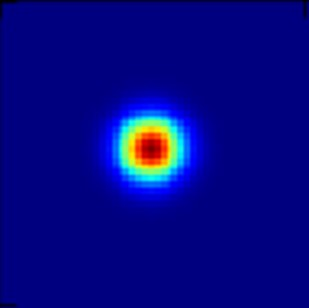
\includegraphics[width=\linewidth]{figures/reference}
\caption{Reference signal}
\label{fig:reference}
\end{minipage}
\hspace{\fill}
\begin{minipage}[t]{0.3\textwidth}
\centering
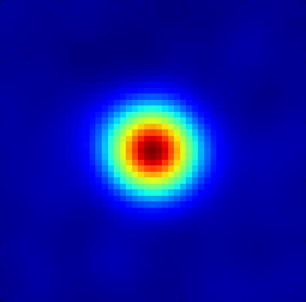
\includegraphics[width=\linewidth]{figures/correlation}
\caption{Correlation result}
\label{fig:correlation}
\end{minipage}
\end{figure}

\section{Comparison Between Methods}

Based on~\cite{thomas04}, the windowing and thresholding methods give similar result, while correlation methods leads to better accuracy at low signal to noise ratio (SNR), in other words, it is more robust for low SNR rather than thresholding and windowing. However correlation process takes high computation effort compared to thresholding and windowing method.

Windowing method has fast calculation process, and very easy to implement. However, this method only compute the centroid in the surrounding of most significant spot. If there are quite significant spots outside the window, they will not be included into the calculation. It can result in not accurate estimation of centroid.

Thresholding method, just like windowing, is easy to implement and has fast calculation process. It can estimate the centroid well, but for low SNR, noise will have big impact on the calculation, which will lead to inaccurate estimation of centroid.

Based on the advantages and disadvantages of each of method, thresholding is regarded as the most suitable method to be used in COntrol for High Resolution Images project because it can give quite accurate estimation with little computational effort.

\section{Wavefront Slopes}

After getting the centroid, we can use that information to determine the wavefront slopes. The gradient of the wavefront can be calculated based on the motion of the centroid of a diffracted spot \cite{spiricon04}. The first process is to calculate the change in the diffacted spot position along the $x$-axis and $y$-axis ($\Delta x$ and $\Delta y$ respectively). They are found by substracting the measured diffracted spot position (obtained from centroid algorithm) from the reference spot positions.

The measured two dimensional wavefront is represented by variable $\Phi(x,y)$, and the slope (gradient) of the wavefront is represented by $\frac{\mathrm{d} \Phi(x,y)}{\mathrm{d} x}$ and $\frac{\mathrm{d} \Phi(x,y)}{\mathrm{d} y}$ for the gradient along $x$-axis and $y$-axis respectively.

\begin{figure}[H]
    \centering
    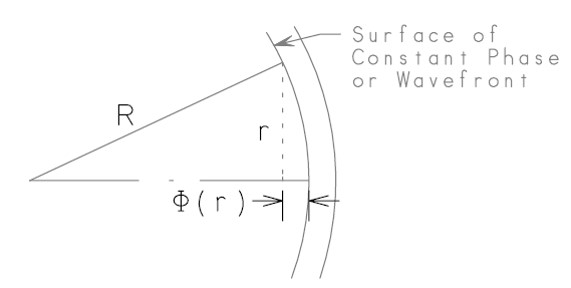
\includegraphics[width=3.5in]{figures/slope1.jpg}
    \caption{Wavefronts with a radius of curvature, $R$, and the phase as a function of radius, $r$, from the optical axis.}
    \label{fig:slope1}
\end{figure}

From the geometry of figure~\ref{fig:slope1}, we can write the equation:

\begin{equation}
R^2=r^2+(R-\phi(2))^2
\end{equation}

Solving for the wave-front $\phi$, we get:



\begin{figure}[H]
    \centering
    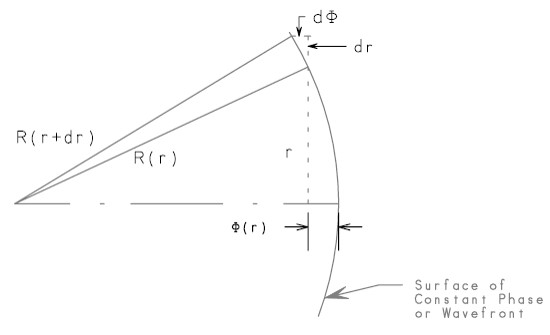
\includegraphics[width=3.5in]{figures/slope2.jpg}
    \caption{The slope of the wave-front}
    \label{fig:slope2}
\end{figure}

\begin{figure}[H]
    \centering
    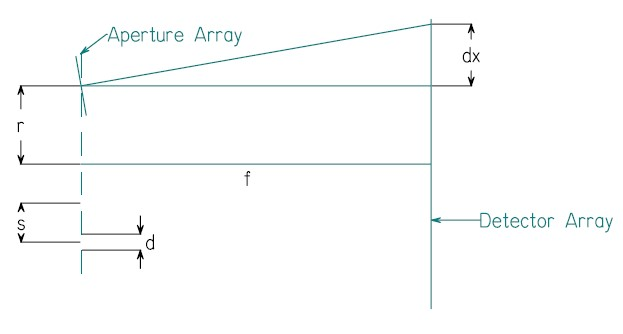
\includegraphics[width=3.5in]{figures/slope3.jpg}
    \caption{The diffraction spot displacement on the detector due to the slope of the wave-front at the aperture array}
    \label{fig:slope3}
\end{figure}

The average gradient of the wavefront over the aperture diameter along the x-axis and y-axis are calculated using equation:

\begin{equation}
\frac{\mathrm{d} \Phi(x,y)}{\mathrm{d} x}=\frac{\Delta x}{f}
\end{equation}

\begin{equation}
\frac{\mathrm{d} \Phi(x,y)}{\mathrm{d} y}=\frac{\Delta y}{f}
\end{equation}
where $f$ is the distance between the aperture array and the detector array \cite{spiricon04}.

\section{Choice of Appertures Mechanism}

Sometimes it is needed to throw away some information(s) of some apertures due to the lack of lighting or the centroid spot cannot be found in the neighborhood of its ideal position. Lack of lighting can make the centroid calculation not accurate, since it means we got low signal to noise ratio. The lighting is so low so that it is difficult to differentiate it to the noise. Based on that, we should throw away information of some apertures with low lighting. To do that we can normalize the intensity values so that its value between 0 and 1. Then specify a certain parameter (also between 0 and 1) as a threshold, which all the intensity(s) below that threshold shold be thrown away due to lack of illumination


\begin{thebibliography}{9}

\bibitem{Verhaegen12}
  M. Verhaegen,
  \emph{Lecture notes on control for High Resolution Imaging}.
  TU Delft, 
  The Netherlands,
  2012.
  
\bibitem{thomas04}
  S. Thomas,
  \emph{Optimized centroid computing in a Shack-Hartmann sensor}.
  SPIE, 
  vol.5490,pp. 1238-1246,
  2004. 
  
\bibitem{spiricon04}
  Spiricon,ed.,
  \emph{Hartmaan Wavefront Analyzer Tutorial}.
  Spiricon, 
  2004.
  
\bibitem{poyneer03}
  L.A. Poyneer, K. LaFortune, A.A.S. Awwal,
  \emph{Correlation wavefront sensing for Shack-Hartmann-based Adaptive Opics with a point source}.
  Lawrence Livermore National Lab Document,
  Livermore, CA 94551
  2003.  

\end{thebibliography}

\end{document}